\chapter{Introduction}
\label{ch:intro}

\begin{quote}
So much of life, it seems to me, is determined by pure randomness –  Sidney Poitier	
\end{quote} 

As Sidney Poitier rightly stated, Randomness determines a great deal of things in life and so do the random numbers.\cite{Charan:2002} 

In the modern era, random numbers play a significant role in many fields, including science, statistics, gaming, security, and many others, for a variety of purposes. For example, computer simulation and modelling complex scenarios in AI systems, where the scenarios are completely unpredictable, selection of random samples from enormous data sets for statistical analysis, data encryption, and games where indiscriminate numbers is very useful, like electronic casino, dice games, etc., are just a few examples.

Speaking about other areas where random numbers are utilized, security and cryptography make great use of them. In cryptography, random numbers are used to create keys, salts, nonces, and other characteristics that make the protocols more unpredictable. Because of its unpredictable nature, it is challenging for an attacker to decrypt a communication without knowing the secret key that was used to encrypt it. To guarantee the quality of the randomness used in cryptographic protocols, it is crucial to utilize a real random number generator.


%
% Section: Need for Random Numbers in Embedded Environment
%
\section{Need for Random Numbers in Embedded Environment}
\label{sec:intro:Need for Random Numbers in Embedded Environment}

The number of connected devices in use today has increased, raising concerns about things like data privacy and unauthorized system access, along with several other things. Because embedded devices are a part of every connected device, their security is essential. 

Another significant business adopting embedded devices, not just embedded devices, but real-time embedded devices is the Automotive industry. One of the greatest markets for real-time embedded devices is the automotive sector. Tens to hundreds of electronic control units are present in every car on the road today, creating potential vulnerabilities for outsiders to enter, alter, and influence the behaviour of the vehicle. Securing the device and every channel via which the communication to the vehicle is made is crucial to prevent any such intrusion into the device.

Considering the importance of random numbers in security from the previous part and the requirement for protecting embedded devices. The significant need for good random numbers in embedded devices may be explained.

%
% Section: Generation of Random Numbers
%
\section{Generation of Random Numbers}
\label{sec:intro:Generation of Random Numbers}

Spoken about random numbers and its importance, it becomes crucial to know how these random numbers are generated and can these be generated in the closed system. Two approaches are available to generate the random numbers.

\begin{itemize}
	\item First approach is based on physical process: This technique produces entirely non-deterministic random numbers. As the gathering process is solely reliant on physical phenomena and results in fully unexpected numbers, this type of generator is known as a non-deterministic random number generator (NRNG) or non-deterministic random bit generator (NRBG).
	\item Second approach is based on deterministic algorithm:  This technique uses random numbers produced by several of the well-known public algorithms. Although though generated numbers appear random, they are entirely random since the algorithm controls everything. As a result, they are often referred to as pseudo random number generators (PRNG), deterministic random number generators (DRNG), or deterministic random bit generators (DRBG).
\end{itemize}

Regular PRNGs cannot provide the kind of random numbers needed for security applications because cryptography demands highly reliable random numbers. There are therefore other PRNGs that are permitted for use in cryptography. Cryptographically Secure Pseudo Random Number Generators (CSPRNG) are the name given to these PRNGs. 

%
% Section: Motivation
%
\section{Motivation}
\label{sec:intro:structure}

NRBGs are ideally suited for cryptography since they create the most unexpected Random Numbers. Nevertheless, not all systems have TRNGs, and it takes a long time to generate random numbers using TRNGs. This makes DRBG in a system necessary. 

In systems lacking TRNG, DRBG is necessary since it generates random numbers more quickly and on demand. But, randomly produced numbers may be predicted. So, to make the random numbers unpredictable, we require a seed input to the DRBG. Random number unpredictability is solely dependent on the seed. Thus, the seed's durability is important. 

TRNGs are a fantastic source of seed, but as was already said, not all systems can support them. This highlights the need for a source that can provide random numbers that can be utilized as a seed for DRBG. Entropy source is the name of this source. Entropy is a measure of a random number's quality or unpredictability. Chapter 2 will provide a comprehensive explanation of entropy, entropy source and available entropy sources. 

The freshness values that the entropy source produces as an output make up most bits in the seed for the DRBG. Nevertheless, using real-time embedded devices has significant disadvantages that make it more difficult to obtain the necessary quantity of entropy.

The following are the fundamental causes of difficulties in extracting sufficient entropy in embedded real-time systems, such as ECU in the automobile domain: 

\begin{itemize}
	\item To determine if enough entropy has been acquired, the amount of entropy created by the source in one sample is unknown.
	\item The absence of sources that are typically accessible in all ECUs.
	\item Each device could not produce the same amount of entropy if common sources are present.
	\item The amount of entropy accessible at start-up is insufficient due to the shorter boot time.
	\item The absence of often changing user interfaces.
	\item Using predefined seeds is often ineffective since they might be compromised. 
\end{itemize}

The general idea of cyber security may deteriorate if there is insufficient entropy. As shown in Figure \ref{fig:1:1}, although if the notion of cyber security is quite solid, if sufficient entropy is not given, it is equivalent to building a massive structure on unstable ground. We are never sure when a structure will crumble.

\begin{figure}[htbp]
	\centering
	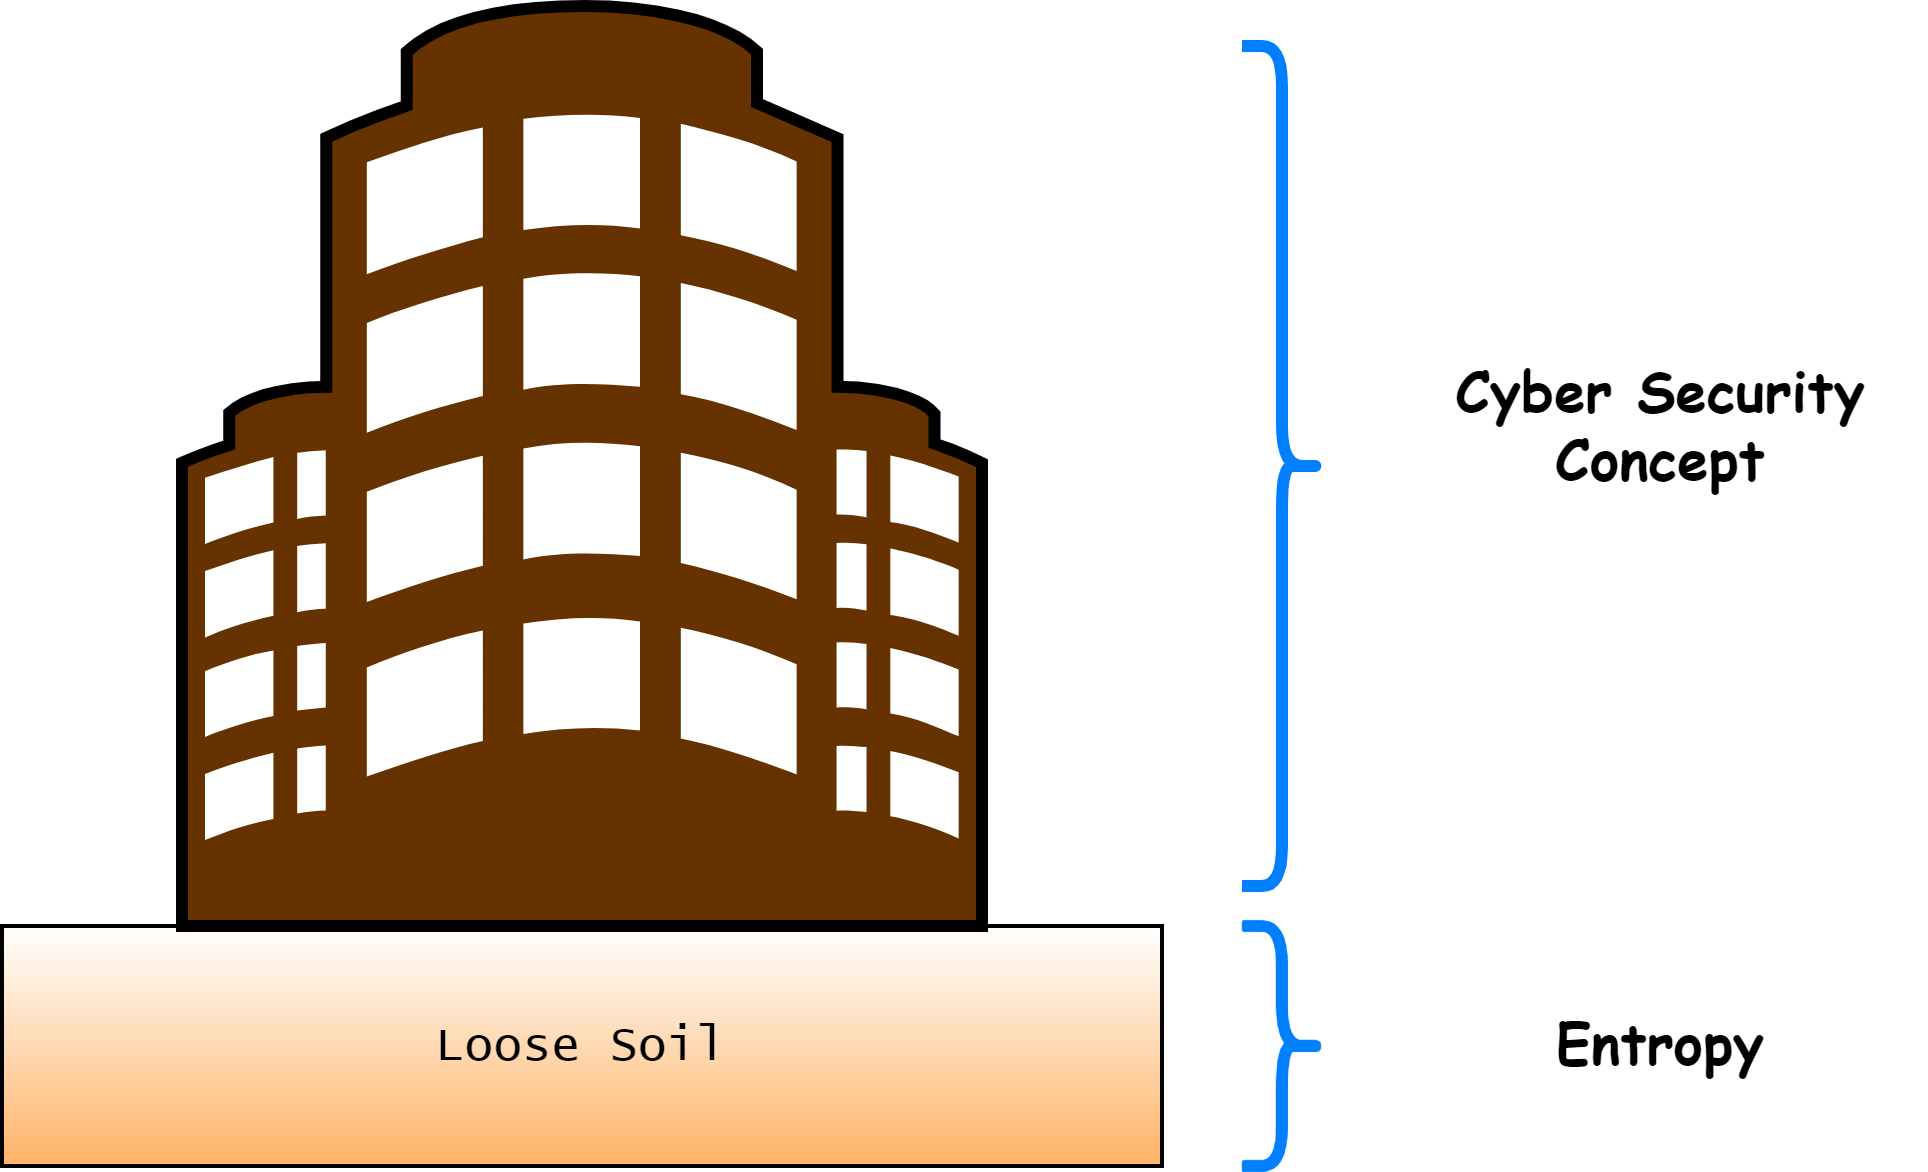
\includegraphics[width=0.75\textwidth]{gfx/diagrams/EffectOfWeakEntropy}
	\caption{Illustration of dependency of security concept on entropy}
	\label{fig:1:1}
\end{figure}

The fact that entropy is a fundamental component of cryptography/security motivates understand more about available entropy sources and ways to enhance the reliability of random numbers in electronic control units (ECUs). Chapter 4 provides a comprehensive discussion of the issues.

%
% Section: Objective
%
\section{Objective}
\label{sec:intro:Objective}

We need a universal remedy that works in all ECUs without TRNG, like HSM, to reduce the frequent problems as seen in the preceding section. The purpose of this thesis is to locate and evaluate potential sources of entropy within the ECU, comprehend the requirements from the NIST SP 800-90 standard series, and design an architecture that aids in gathering enough entropy from sources for the system to be secure and to manage the boot time entropy requirement. 

Furthermore, a UI-based framework must be designed and developed to automatically produce code in accordance with the proposed architecture based on NIST standards. The framework should be able to record the following user inputs:

\begin{itemize}
	\item Required security strength.
	\item Selection of entropy sources.
	\item Scheduling entropy collection from sources.
	\item Runtime validation of the entropy sources.
\end{itemize}

The framework's ability to produce code that is ready for integration based on user inputs should be evaluated and confirmed. The final product of the created code should behave like a TRNG and provide high-quality random numbers that can be seeded into DRBG to produce the random numbers.

The entropy source’s operational circumstances and attack vectors must be determined. Subsequently, techniques must be created to mitigate circumstances under which, random numbers are compromised for any cause, weakening the security.

%
% Section: Working Environment
%
\section{Working Environment}
\label{sec:intro:Working Environment}

The thesis is written in cooperation with Automotive Cybersecurity team at Bosch Engineering GmbH (BEG). BEG is a fully owned subsidiary of Robert Bosch GmbH that specializes in the modifying of Bosch high-volume technology. BEG delivers improvements for car and engine manufacturers. The business has 1,550 employees and is based in Abstatt.

Automotive Cybersecurity team at BEG concentrates on analysis of security threats,  development of security concepts and engineering the concepts for a customer. 

%
% Section: Thesis Outline
%
\section{Thesis Outlinet}
\label{sec:intro:Thesis Outline}

The following sentences provide a summary of this thesis and its organization before getting into further detail:

\begin{description}
	\item[Chapter 2 (Fundamentals)] The essentials, including entropy, different forms of entropy, and other terminology, are covered in this chapter.
	\item[Chapter 3 (State of Art)] Here, we try to comprehend earlier studies on a related subject. Explain the pooling algorithms that the standard recommends for embedded systems, including Fortuna and Linux RNG.
	\item[Chapter 4 (Conceptual Design)] In this chapter, we go into detail about the issue statement and outline the requirements based on it and the elements of the problem statement that cannot be handled using the State of the Art at this time. An explanation of the concept's architecture, a justification of how the idea solves the issue indicated in the reason. Provide a design for Framework.
	\item[Chapter 5 (Implementation)] The implementation of the notion that is discussed in Chapter 4 is attempted to be described in this chapter. explains each component of the Framework, how it was used, and how to incorporate it into current applications.
	\item[Chapter 6 (Results and Analysis)] This chapter analyzes the architectural design, outlining its benefits and shortcomings and evaluates the target entropy's risk.
	\item[Chapter 7 (Outline and conclusion)] This chapter concludes the Thesis with the recommendations and future work which can/needs to be done.
\end{description}


